\subsection{Simulación del Modelo de Consumo}

La simulación del modelo de consumo energético se realiza mediante un proceso estructurado que incluye la carga y procesamiento de datos de telemetría, la optimización de parámetros del modelo, la comparación con datos reales, y el análisis de consumo y emisiones. A continuación se describe detalladamente cada etapa del proceso de simulación.

\subsubsection{Procesamiento de Datos de Telemetría}

La simulación comienza con la carga de datos de telemetría desde un archivo JSON que contiene información de múltiples rutas. Cada ruta se identifica mediante un campo de identificación, y se selecciona la ruta más larga para el análisis. Los datos de telemetría incluyen:

\begin{itemize}
    \item Corriente eléctrica ($i_A$) en amperios
    \item Coordenadas GPS (latitud, longitud)
    \item Altitud en metros
    \item Velocidad en km/h ($spdKmh$)
    \item Timestamps en milisegundos
\end{itemize}

A partir de la corriente eléctrica y asumiendo un voltaje de $48$ V, se calcula la potencia real consumida mediante $P_{\mathrm{real}} = i_A \times 48$ V. Las Figuras \ref{fig:telemetria_electrica}, \ref{fig:telemetria_gps} y \ref{fig:telemetria_velocidad} muestran los datos de telemetría organizados en grupos temáticos.

\paragraph{Parámetros Eléctricos}

Las Figuras \ref{fig:telemetria_corriente_potencia} y \ref{fig:telemetria_soc} muestran los parámetros eléctricos de la motocicleta durante la ruta.

\begin{figure}[htbp]
\centering
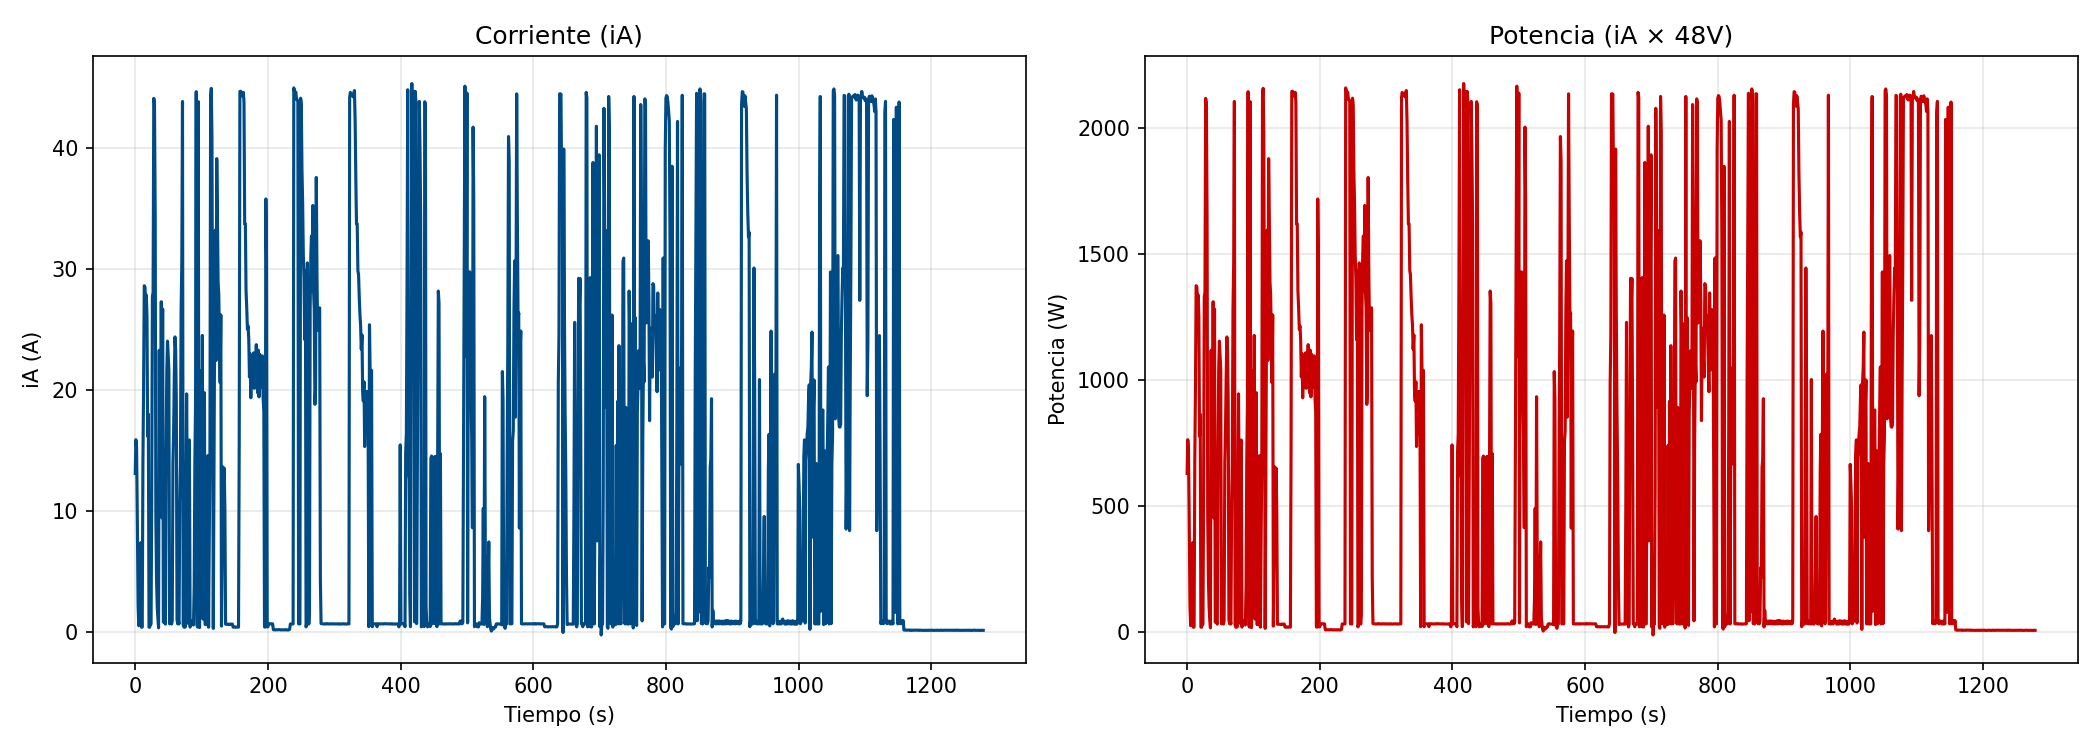
\includegraphics[width=0.95\textwidth]{telemetria_corriente_potencia.png}
\caption{Parámetros eléctricos de telemetría: (a) Corriente eléctrica y (b) Potencia calculada.}
\label{fig:telemetria_corriente_potencia}
\end{figure}

La gráfica de corriente eléctrica muestra las variaciones de consumo de corriente a lo largo del tiempo (en segundos), mientras que la potencia se calcula directamente como el producto de corriente y voltaje.

\begin{figure}[htbp]
\centering
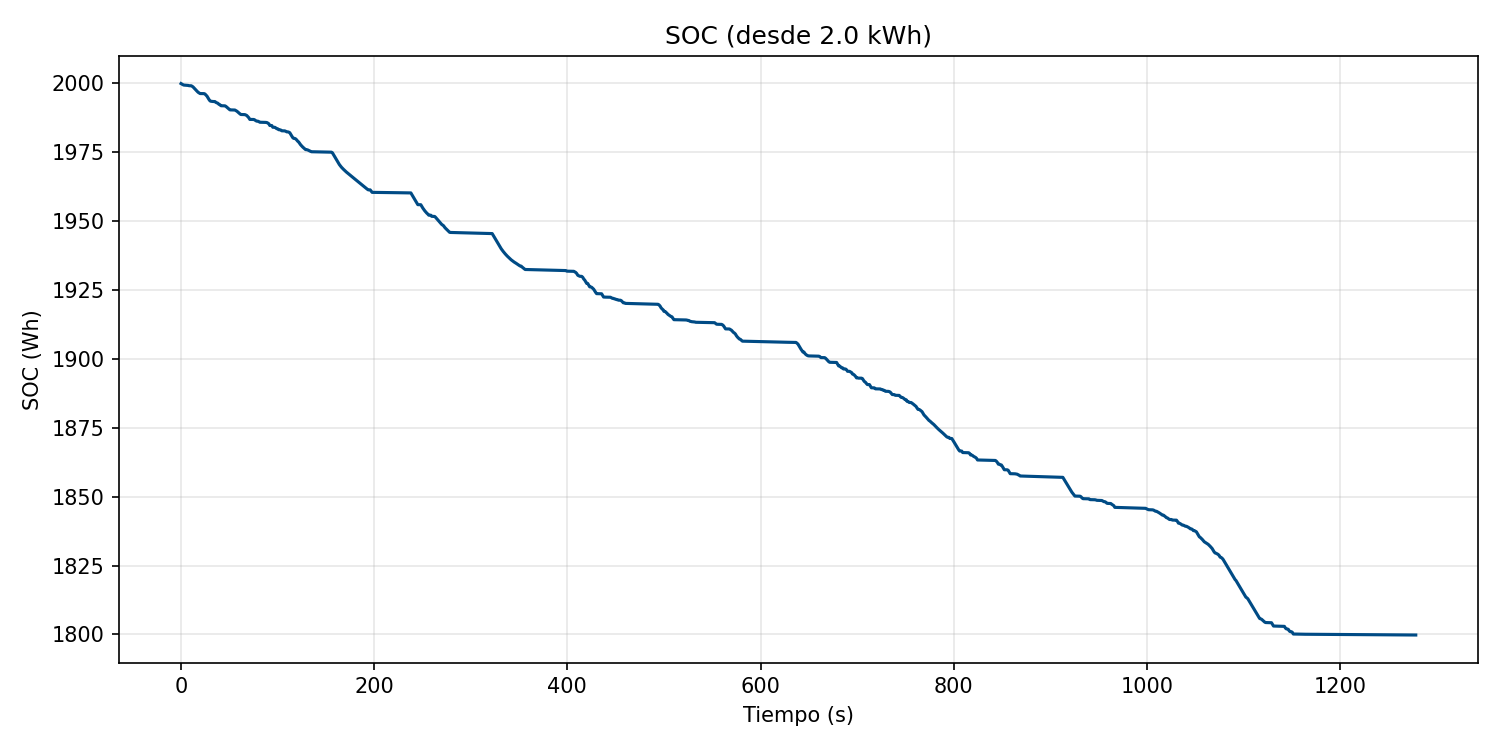
\includegraphics[width=0.7\textwidth]{telemetria_soc.png}
\caption{Estado de carga (SOC) de la batería calculado mediante integración temporal de la potencia consumida, partiendo de una energía inicial de $2000$ Wh.}
\label{fig:telemetria_soc}
\end{figure}

El estado de carga (SOC) se calcula mediante integración temporal de la potencia consumida, partiendo de una energía inicial de $2000$ Wh. El eje horizontal representa el tiempo transcurrido desde el inicio de la ruta en segundos.

\paragraph{Coordenadas Geográficas}

Las Figuras \ref{fig:telemetria_latitud_longitud} y \ref{fig:telemetria_altitud_trayectoria} muestran las coordenadas geográficas y la trayectoria GPS de la ruta.

\begin{figure}[htbp]
\centering
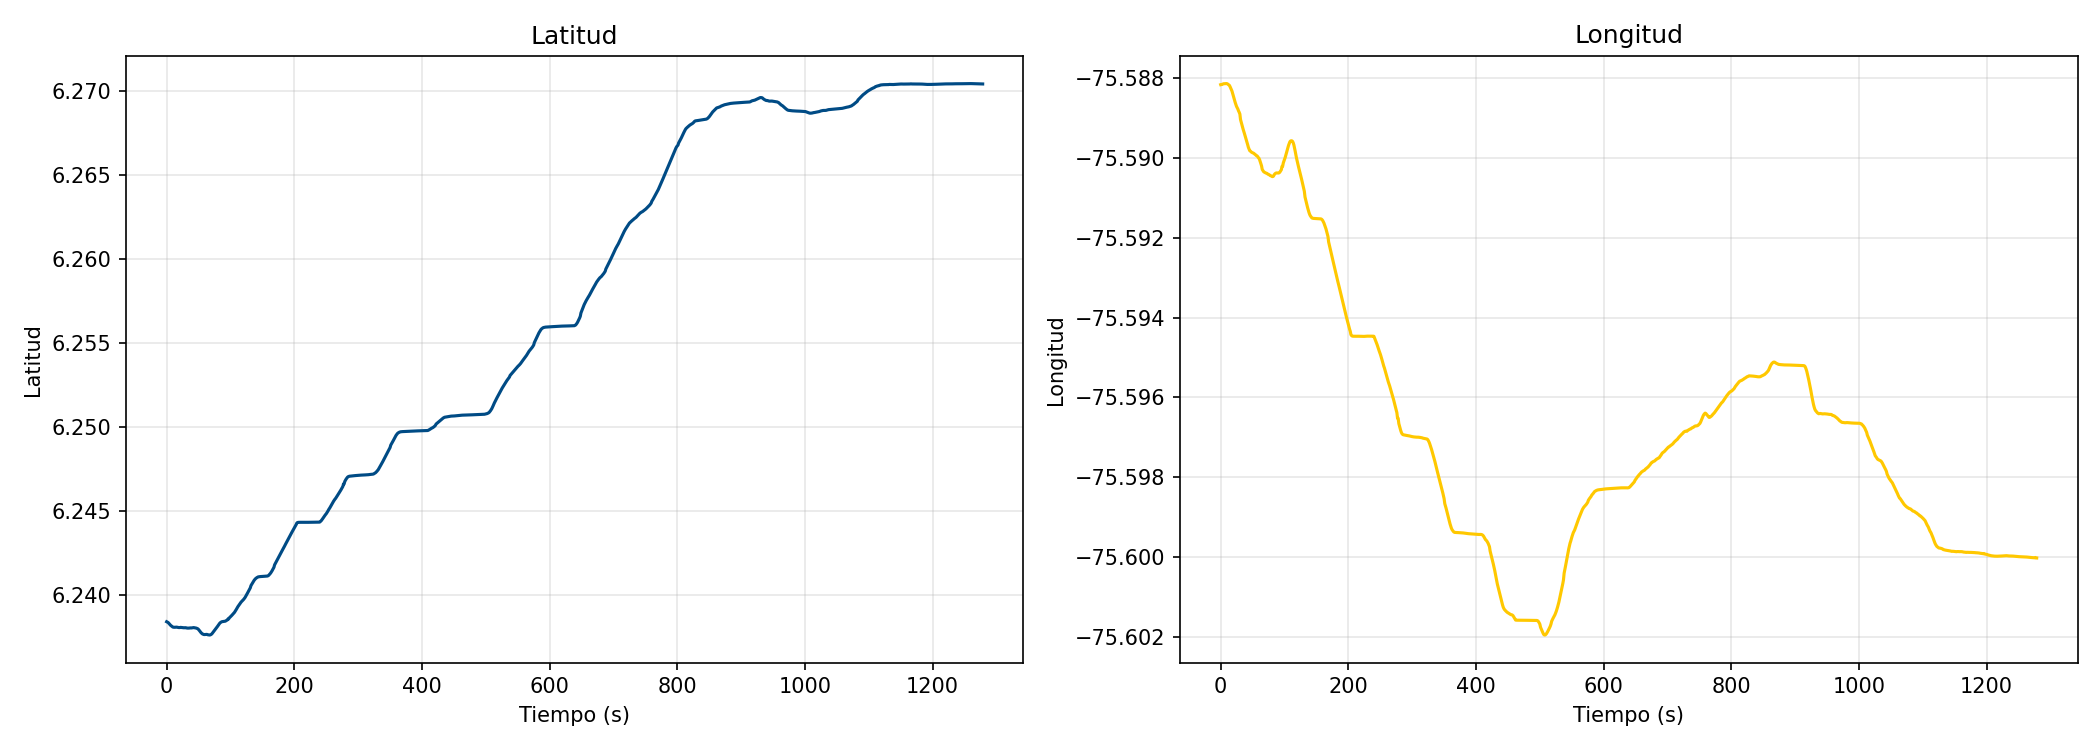
\includegraphics[width=0.95\textwidth]{telemetria_latitud_longitud.png}
\caption{Coordenadas geográficas de telemetría: (a) Latitud y (b) Longitud.}
\label{fig:telemetria_latitud_longitud}
\end{figure}

Las coordenadas de latitud y longitud permiten localizar geográficamente cada punto de la ruta.

\begin{figure}[htbp]
\centering
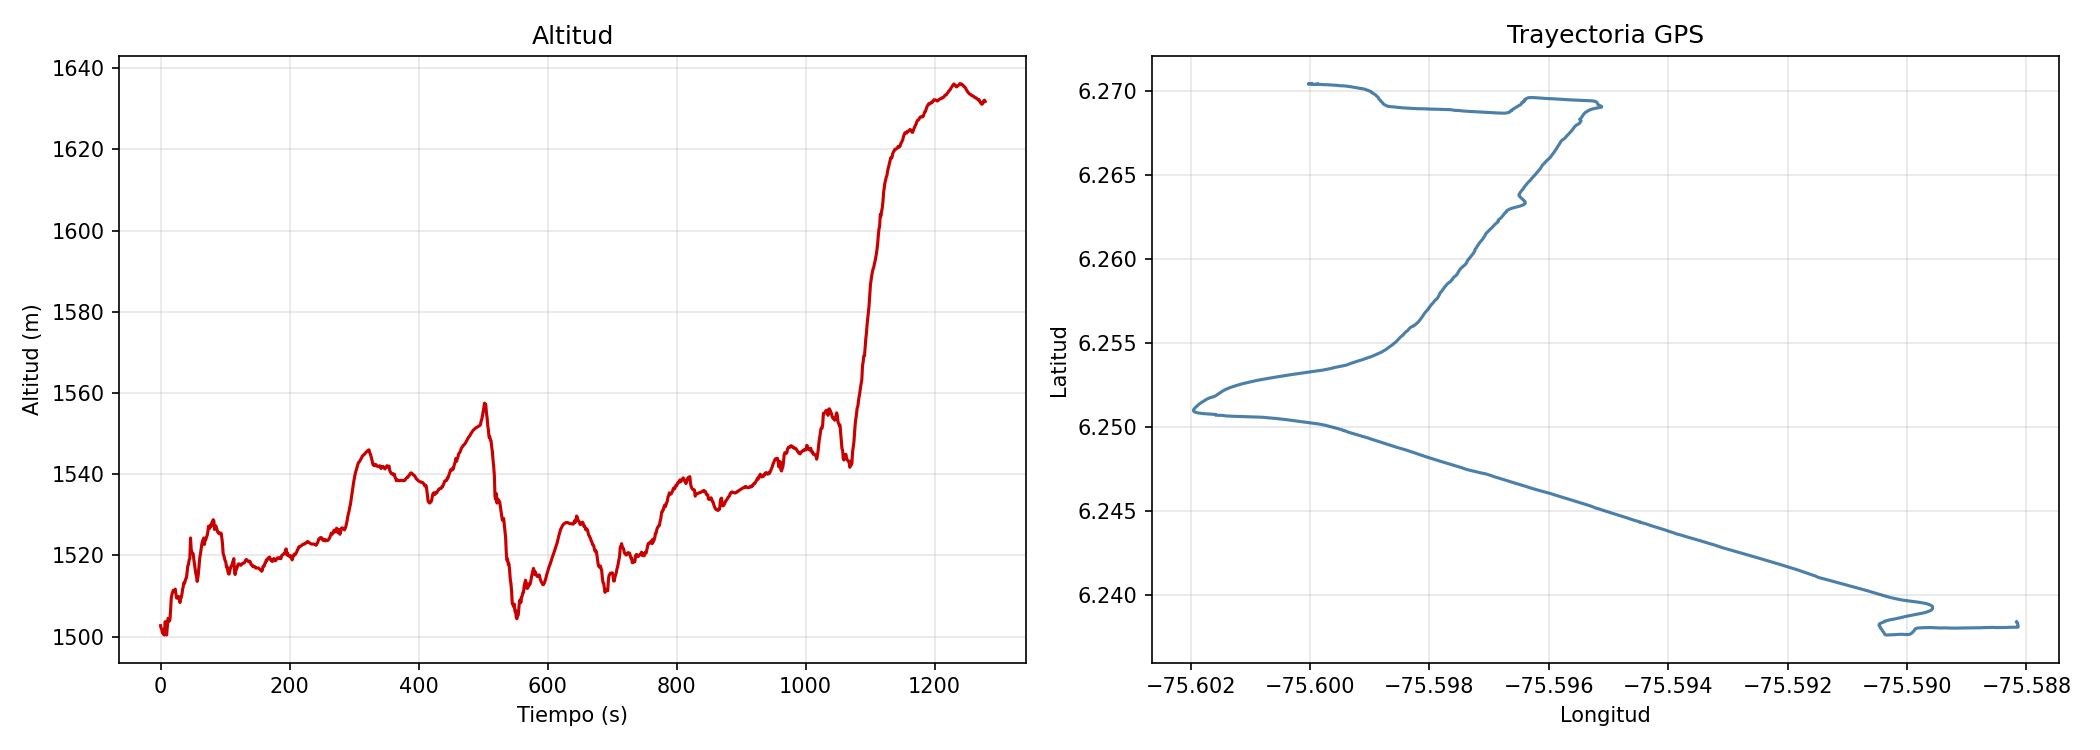
\includegraphics[width=0.95\textwidth]{telemetria_altitud_trayectoria.png}
\caption{Perfil topográfico y trayectoria GPS: (a) Altitud y (b) Trayectoria GPS.}
\label{fig:telemetria_altitud_trayectoria}
\end{figure}

La altitud proporciona información sobre el perfil topográfico de la ruta, mientras que la trayectoria GPS muestra la ruta completa en el plano geográfico.

\paragraph{Parámetros de Movimiento}

La Figura \ref{fig:telemetria_velocidad} muestra la velocidad de la motocicleta durante la ruta.

\begin{figure}[htbp]
\centering
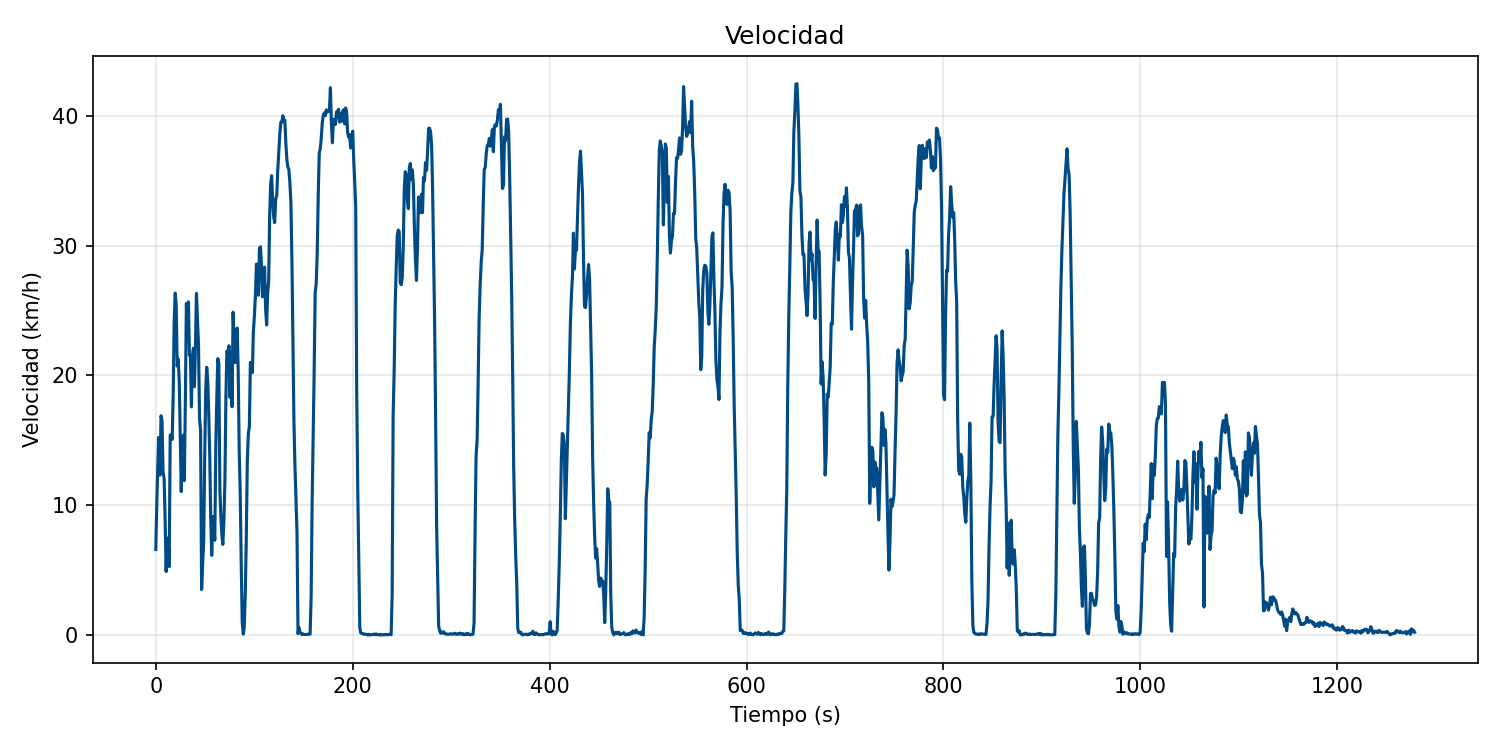
\includegraphics[width=0.7\textwidth]{telemetria_velocidad.png}
\caption{Velocidad de la motocicleta durante la ruta medida en km/h.}
\label{fig:telemetria_velocidad}
\end{figure}

La velocidad se mide directamente mediante el sensor GPS y se registra en km/h, proporcionando información sobre el perfil de velocidad de la ruta.

\subsubsection{Preprocesamiento y Interpolación}

Para mejorar la resolución temporal del modelo y obtener una representación más suave de las variaciones en velocidad y pendiente, se realiza una interpolación lineal de los vectores de datos. El proceso de interpolación genera puntos intermedios entre cada par de puntos originales, aumentando la densidad de datos y permitiendo una simulación más precisa.

El ángulo de inclinación de la carretera se calcula a partir de los datos de altitud GPS mediante la fórmula de Haversine para determinar la distancia horizontal entre puntos consecutivos, y luego se calcula el ángulo mediante la función arco tangente de la relación entre el cambio de altitud y la distancia horizontal.

\subsubsection{Optimización de Parámetros}

Los parámetros del modelo se optimizan mediante minimización del error cuadrático medio entre las predicciones del modelo y las mediciones reales de telemetría. La función objetivo considera tanto el error en potencia como el error en estado de carga (SOC) de la batería. La optimización se realiza mediante el método L-BFGS-B con restricciones de límites para cada parámetro.

Los parámetros optimizados incluyen: masa del vehículo ($m$), coeficiente de arrastre aerodinámico ($c_{\mathrm{d}}$), área frontal ($A$), coeficiente de resistencia a la rodadura ($c_{\mathrm{rr}}$), factor de corrección empírico ($\phi_{\mathrm{corr}}$), y eficiencia del tren de potencia ($\mu_{\mathrm{tren}}$). La Tabla \ref{tab:params_optimizados} muestra los valores típicos de estos parámetros después de la optimización.

\begin{table}[htbp]
\caption{Parámetros optimizados del modelo}
\begin{center}
\begin{tabular}{|c|c|c|}
\hline
\textbf{\textit{Parámetro}} & \textbf{\textit{Símbolo}} & \textbf{\textit{Rango de Optimización}}\\
\cline{1-3} 
\hline
Masa & $m$ & 50 - 200 [kg] \\
Coef. arrastre & $c_{\mathrm{d}}$ & 0.1 - 1.0 \\
Área frontal & $A$ & 0.3 - 1.5 [m²] \\
Coef. rodamiento & $c_{\mathrm{rr}}$ & 0.005 - 0.05 \\
Factor corrección & $\phi_{\mathrm{corr}}$ & 0.5 - 3.0 \\
Eficiencia tren & $\mu_{\mathrm{tren}}$ & 0.6 - 0.95 \\
\hline
\end{tabular}
\label{tab:params_optimizados}
\end{center}
\end{table}

\subsubsection{Resultados de la Simulación}

Los resultados de la simulación se presentan en grupos temáticos que facilitan el análisis y la interpretación de los datos.

\paragraph{Validación del Modelo}

La Figura \ref{fig:validacion_modelo} muestra la comparación entre las predicciones del modelo y los datos reales de telemetría para potencia y estado de carga.

\begin{figure}[htbp]
\centering
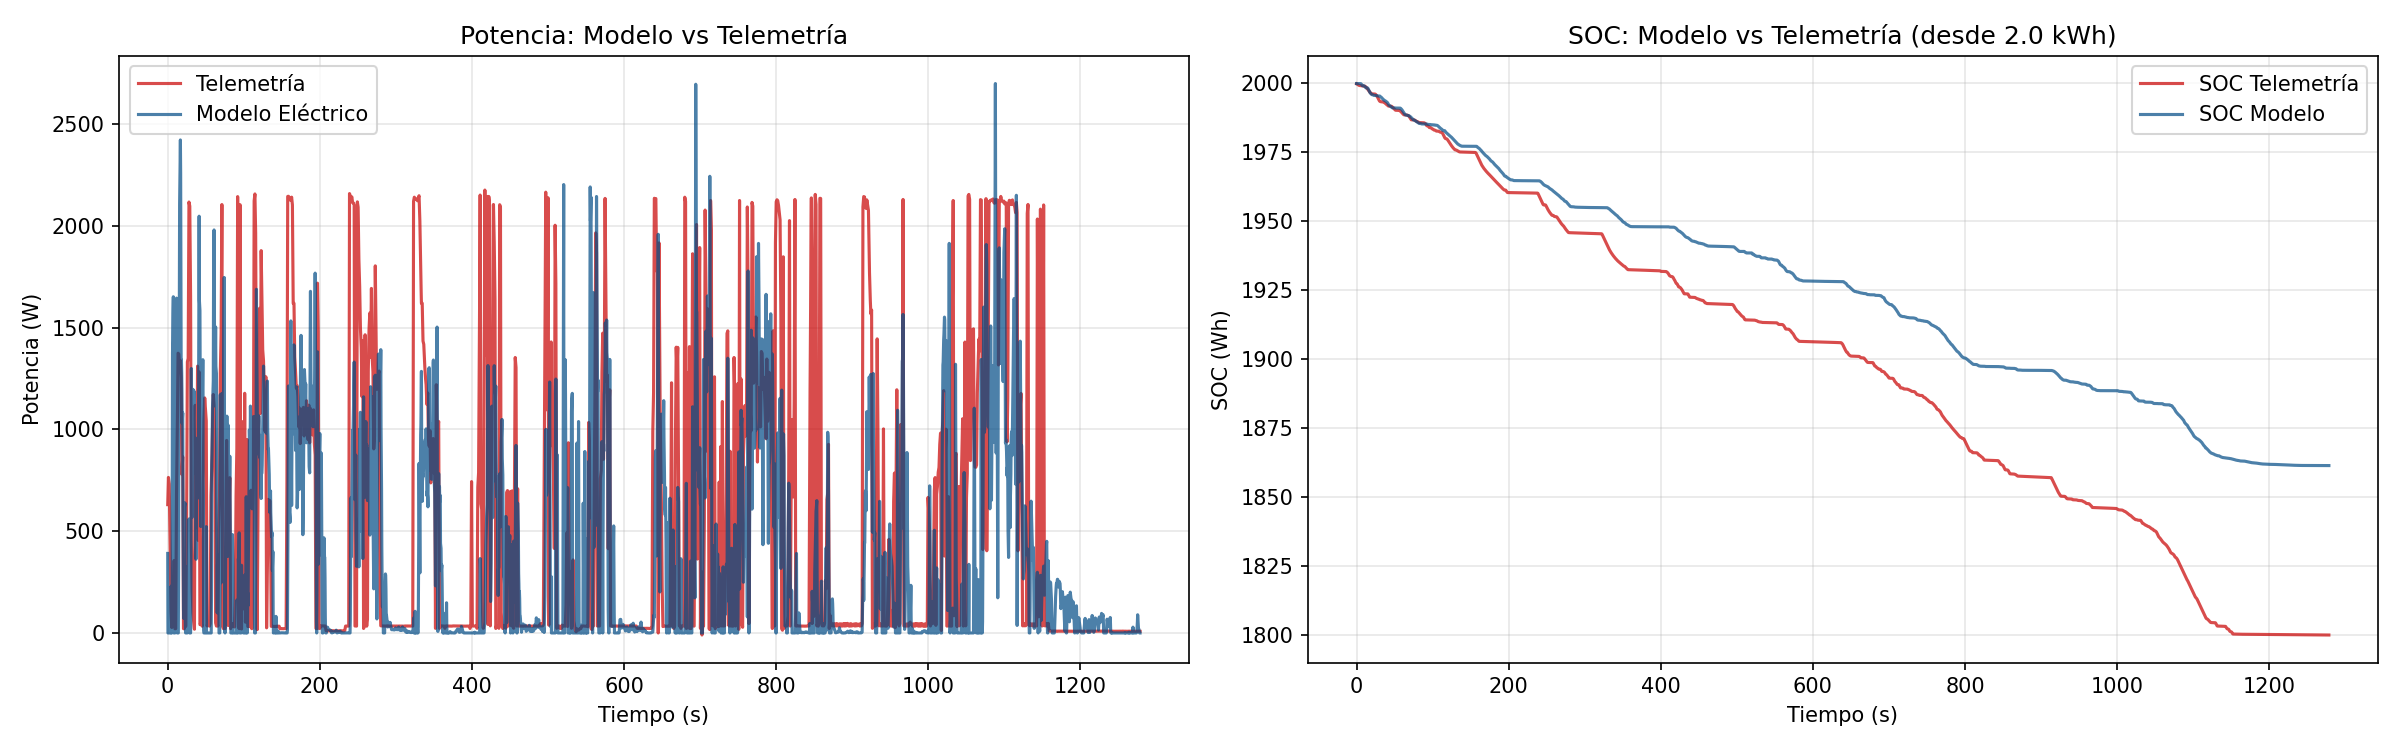
\includegraphics[width=0.95\textwidth]{modelo_validacion.png}
\caption{Validación del modelo: (a) Comparación de potencia entre modelo y telemetría, (b) Comparación de SOC entre modelo y telemetría.}
\label{fig:validacion_modelo}
\end{figure}

La primera gráfica muestra la comparación entre la potencia predicha por el modelo y la potencia medida mediante telemetría en función del tiempo (en segundos). Esta comparación permite validar la precisión del modelo y identificar posibles desviaciones. La segunda gráfica muestra la comparación del estado de carga (SOC) de la batería, calculado mediante integración temporal de la potencia consumida, partiendo de una energía inicial de $2000$ Wh. Estas comparaciones son fundamentales para evaluar la calidad del ajuste del modelo a los datos reales.

\paragraph{Comparación de Tecnologías}

La Figura \ref{fig:comparacion_tecnologias} compara el consumo energético entre una motocicleta eléctrica y una de combustión.

\begin{figure}[htbp]
\centering
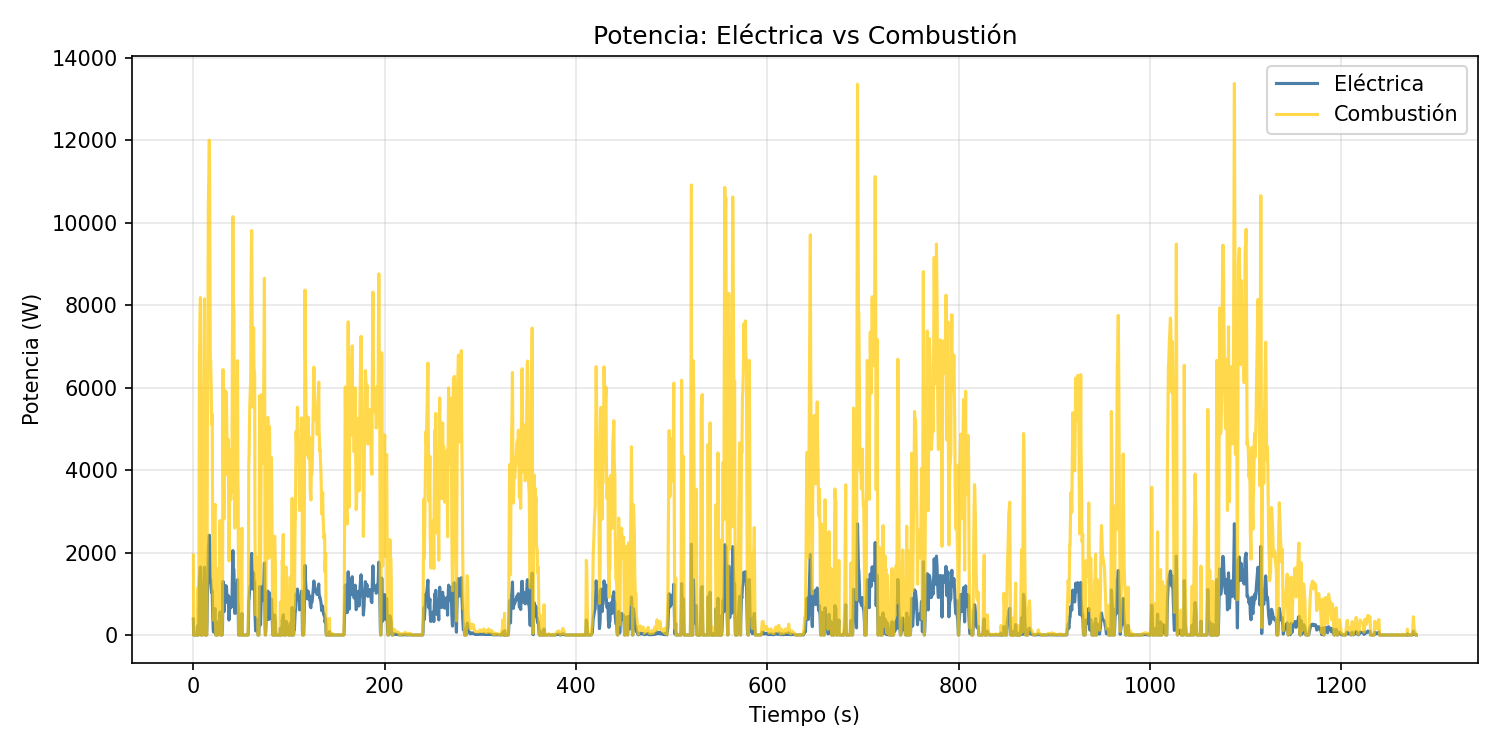
\includegraphics[width=0.7\textwidth]{modelo_comparacion_tecnologias.png}
\caption{Comparación de potencia requerida entre motocicleta eléctrica y de combustión.}
\label{fig:comparacion_tecnologias}
\end{figure}

Esta gráfica compara la potencia requerida por una motocicleta completamente eléctrica ($\alpha_{\mathrm{comb}} = 0$) versus una motocicleta completamente a combustión ($\alpha_{\mathrm{comb}} = 1$) en función del tiempo (en segundos). Esta comparación permite evaluar las diferencias en el consumo energético entre ambas tecnologías bajo las mismas condiciones de ruta, proporcionando información valiosa para la toma de decisiones sobre la elección de tecnología de propulsión.

\paragraph{Análisis Espacial y Temporal}

La Figura \ref{fig:analisis_espacial} muestra la visualización espacial y temporal de la ruta.

\begin{figure}[htbp]
\centering
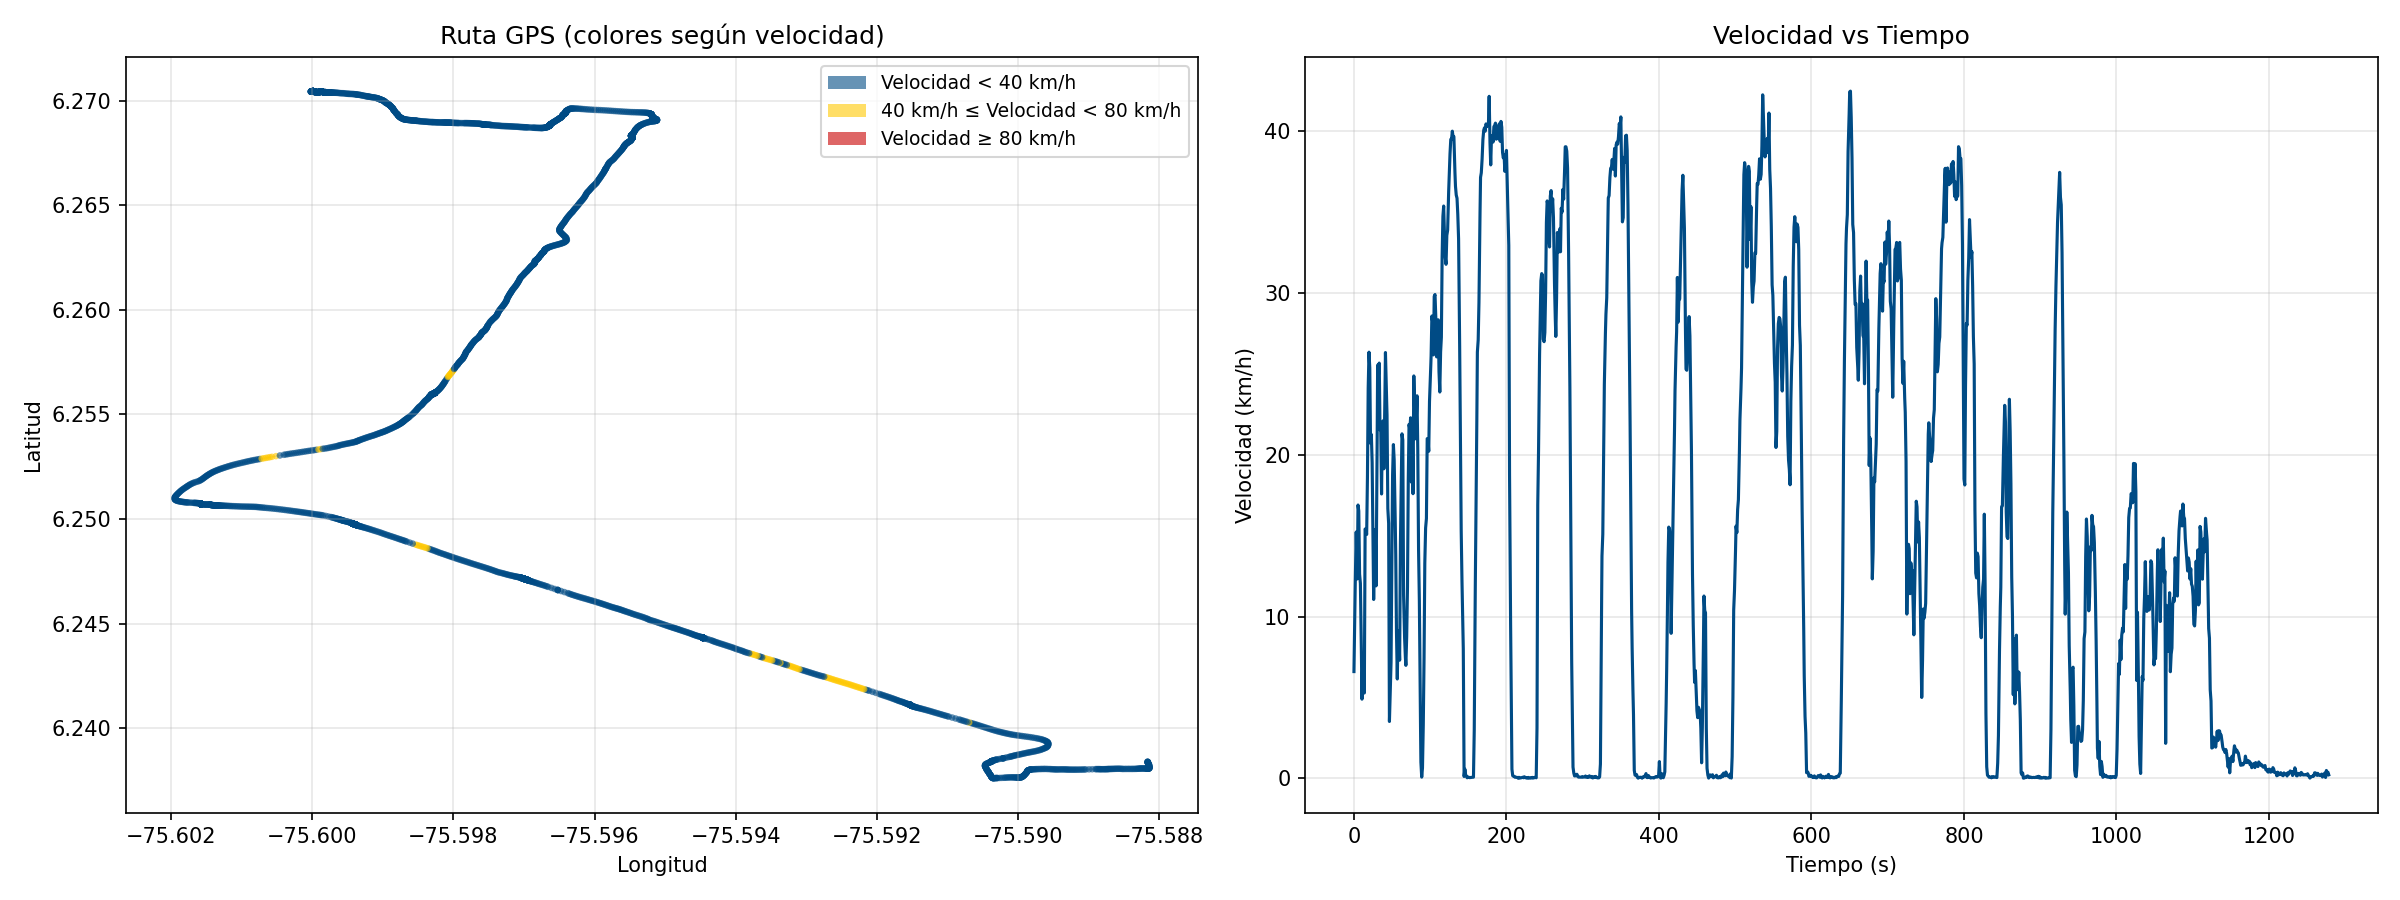
\includegraphics[width=0.95\textwidth]{modelo_analisis_espacial.png}
\caption{Análisis espacial y temporal: (a) Ruta GPS con colores según velocidad, (b) Velocidad vs tiempo.}
\label{fig:analisis_espacial}
\end{figure}

La primera gráfica muestra la ruta GPS con colores que indican la velocidad en cada punto según los siguientes rangos: azul para velocidades menores a $40$ km/h, amarillo para velocidades entre $40$ y $80$ km/h, y rojo para velocidades mayores o iguales a $80$ km/h. La leyenda en la gráfica permite identificar fácilmente estos rangos de velocidad, facilitando la interpretación de los tramos de la ruta. Los tramos amarillos corresponden a velocidades moderadas entre $40$ y $80$ km/h, típicas de tráfico urbano fluido o carreteras secundarias. La segunda gráfica muestra la velocidad en función del tiempo, proporcionando información sobre el perfil de velocidad de la ruta y permitiendo identificar períodos de aceleración, velocidad constante y desaceleración.

\paragraph{Análisis de Emisiones}

La Figura \ref{fig:emisiones} muestra una comparación de las emisiones equivalentes de ciclo de vida.

\begin{figure}[htbp]
\centering
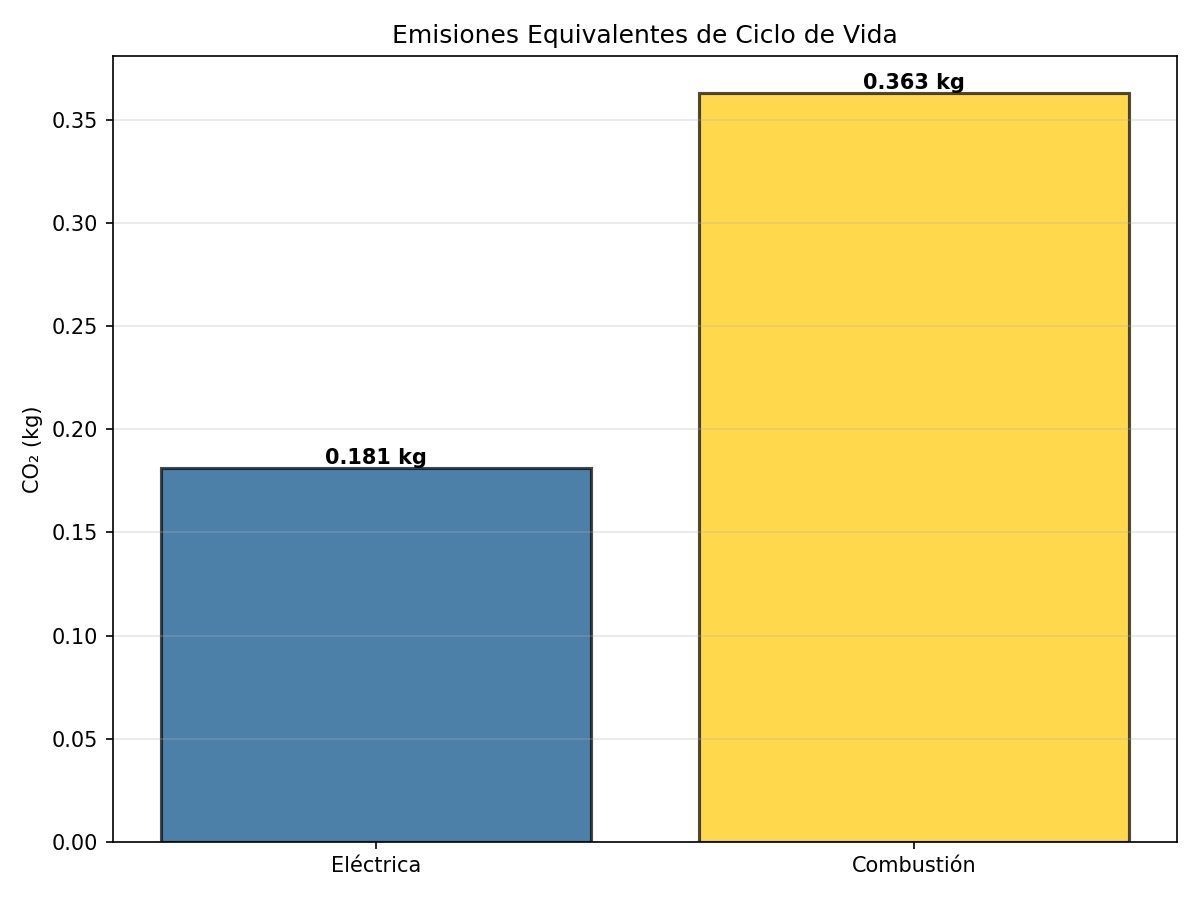
\includegraphics[width=0.6\textwidth]{modelo_emisiones.png}
\caption{Comparación de emisiones equivalentes de ciclo de vida entre motocicleta eléctrica y de combustión.}
\label{fig:emisiones}
\end{figure}

Esta gráfica muestra una comparación de las emisiones equivalentes de ciclo de vida entre una motocicleta eléctrica y una de combustión. Las emisiones se calculan mediante factores de emisión específicos: $35$ gCO$_2$/km para motocicletas eléctricas y $70$ gCO$_2$/km para motocicletas de combustión, considerando todo el ciclo de vida del vehículo y la generación de energía. Esta comparación permite cuantificar el beneficio ambiental de la tecnología eléctrica.

\subsubsection{Métricas de Validación del Modelo}

Para evaluar la precisión del modelo, se calculan diversas métricas de error y correlación. La Tabla \ref{tab:metricas_validacion} muestra las métricas típicas obtenidas de la simulación.

\begin{table}[htbp]
\caption{Métricas de validación del modelo}
\begin{center}
\begin{tabular}{|c|c|}
\hline
\textbf{\textit{Métrica}} & \textbf{\textit{Descripción}}\\
\cline{1-2} 
\hline
Error medio potencia & Error absoluto medio entre potencia modelo y real \\
Error porcentual medio potencia & Error porcentual medio de potencia \\
Correlación potencia & Coeficiente de correlación de Pearson \\
Error medio SOC & Error absoluto medio entre SOC modelo y real \\
Error porcentual medio SOC & Error porcentual medio de SOC \\
Correlación SOC & Coeficiente de correlación de Pearson para SOC \\
\hline
\end{tabular}
\label{tab:metricas_validacion}
\end{center}
\end{table}

Estas métricas permiten cuantificar la calidad del ajuste del modelo a los datos reales y identificar áreas de mejora en la calibración de parámetros.

\subsubsection{Resultados de Consumo y Emisiones}

La simulación calcula el consumo energético total y las emisiones equivalentes de ciclo de vida para ambas configuraciones (eléctrica y combustión). La Tabla \ref{tab:resultados_consumo} muestra un ejemplo de los resultados típicos obtenidos.

\begin{table}[htbp]
\caption{Resultados de consumo y emisiones}
\begin{center}
\begin{tabular}{|c|c|c|}
\hline
\textbf{\textit{Parámetro}} & \textbf{\textit{Eléctrica}} & \textbf{\textit{Combustión}}\\
\cline{1-3} 
\hline
Consumo energético & Variable [kWh] & Variable [kWh] \\
Consumo combustible & - & Variable [galones] \\
Factor emisión & 35 [gCO$_2$/km] & 70 [gCO$_2$/km] \\
Emisiones totales & Variable [kg CO$_2$] & Variable [kg CO$_2$] \\
\hline
\end{tabular}
\label{tab:resultados_consumo}
\end{center}
\end{table}

El consumo de combustible en galones se calcula mediante la conversión del consumo energético de combustión utilizando el poder calorífico de la gasolina ($33.7$ kWh/galón). La reducción porcentual de emisiones se calcula comparando las emisiones de la configuración eléctrica con las de la configuración de combustión.

\subsubsection{Mapa Interactivo de la Ruta}

Adicionalmente, la simulación genera un mapa HTML interactivo que muestra la ruta realizada con información detallada en cada punto. El mapa incluye:

\begin{itemize}
    \item Visualización de la ruta con colores según velocidad
    \item Marcadores de inicio y fin de la ruta
    \item Puntos intermedios con información de velocidad, altitud y potencia
    \item Panel de información con resumen de consumo y emisiones
    \item Leyenda de colores para interpretación de velocidades
    \item Capas de mapa base y satelital
\end{itemize}

Este mapa interactivo permite una visualización detallada de la ruta y facilita el análisis espacial de los datos de consumo y velocidad.

\subsubsection{Resumen de la Simulación}

La simulación completa del modelo de consumo energético proporciona una herramienta integral para:

\begin{enumerate}
    \item Validar el modelo matemático mediante comparación con datos reales de telemetría
    \item Optimizar los parámetros del modelo para mejorar la precisión de las predicciones
    \item Comparar el rendimiento entre configuraciones eléctricas y de combustión
    \item Analizar el consumo energético y las emisiones equivalentes de ciclo de vida
    \item Visualizar espacialmente la ruta y los datos asociados mediante mapas interactivos
\end{enumerate}

Los resultados de la simulación demuestran la capacidad del modelo para predecir con precisión el consumo energético de la motocicleta eléctrica, así como para realizar comparaciones cuantitativas entre diferentes tecnologías de propulsión. La integración de datos de telemetría real, optimización de parámetros, y análisis de emisiones proporciona una base sólida para la evaluación del rendimiento energético y ambiental de vehículos eléctricos.

